\section{Experimental Comparison}\label{sec:experimental-comparison}

The three loss functions presented in Section~\ref{sec:loss-functions} were experimentally evaluated on 18 publicly available datasets and on a corporate dataset from the domain of computer security. The 2 metrics presented in Section~\ref{sec:clustering-metrics} were used, i.e. the Silhouette coefficient and the accuracy of a kNN classifier built on the embedding. Both of these metrics were tracked over the learning period to also evaluate how the models are learning in addition to their final performance.

\subsection{Datasets}

The evaluation was done on a set of 18 publicly available datasets, listed in Table~\ref{tab:datasets}. All the datasets as used were also made public\footnote{https://github.com/marekdedic/MilDatasets.jl}.

\begin{table}
  \centering
  \begin{tabular}{ll}
    \toprule
    Source & Datasets \\
    \midrule
    \cite{briggs_rank-loss_2012} & BrownCreeper, WinterWren \\
    \cite{andrews_support_2002} & Elephant, Fox, Tiger \\
    \cite{dietterich_solving_1997} & Musk1, Musk2 \\
    \cite{srinivasan_comparing_1995} & Mutagenesis1, Mutagenesis2 \\
    \cite{zhou_multi-instance_2008} & Newsgroups1, Newsgroups2, Newsgroups3 \\
    \cite{ray_learning_2005, ray_supervised_2005} & Protein \\
    \cite{kandemir_empowering_2014} & UCSBBreastCancer \\
    \cite{zhou_multi-instance_2005} & Web1, Web2, Web3, Web4 \\
    \bottomrule
  \end{tabular}
  \caption{The 18 publicly available datasets used.}\label{tab:datasets}
\end{table}

The models were also evaluated on a proprietary dataset provided by Cisco Cognitive Intelligence, consisting of records of network connections from clients (e.g. user computers or mobile devices) to some on-line services. The dataset represents HTTP traffic of more than 100 companies. Two datasets were collected, each spanning 1 day of traffic. The training data was traffic from 2019-11-18, while the data used for testing was collected the following day, 2019-11-19. For each connection, a proprietary classification system based on \cite{jusko_graph-based_2017} provided labels, classifying the connections either as legitimate or malicious (connected to malware activity). The data was sampled to include 90\% of negative bags and 10\% of positive bags. For each connection, 20 connection features were used, as well as a MIL model of the server URL, which is visualized in Figure~\ref{fig:URL-model}.

\begin{figure*}
  \centering
  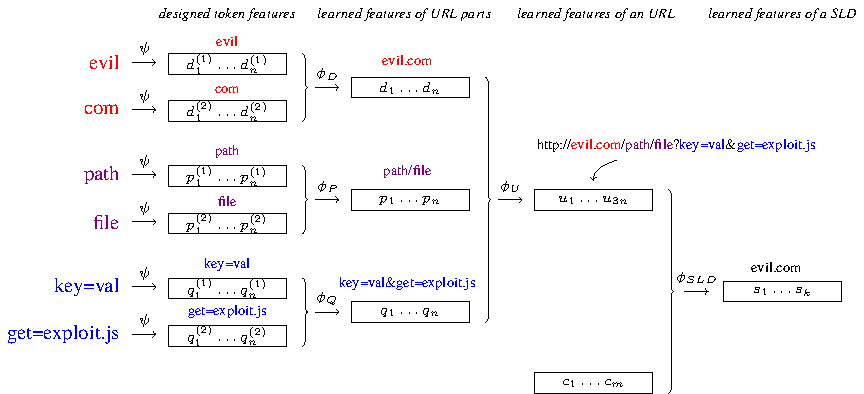
\includegraphics[width=0.8\textwidth]{images/URL-model/URL-model.pdf}
  \caption{Hierarchical model of a URL. The vector \( c_1, \dots, c_m \) represents the connection features.}\label{fig:URL-model}
\end{figure*}

\subsection{Experimental Design}

The models for evaluation were implemented in the Julia programming language \cite{bezanson_julia:_2017} using the Flux.jl framework for machine learning \cite{innes_flux:_2018} and the Mill.jl framework for multi-instance learning\footnote{https://github.com/pevnak/Mill.jl}.

The particular architecture of the models was chosen based upon previous experience with using neural networks in multi-instance setting \cite{pevny_nested_2020}. Several architectures were tested and the best one selected for the experiments. The embedding \( \phi \) was realised by a MIL neural network consisting of 2 per-instance layers of 30 neurons, followed by aggregation formed by concatenating element-wise mean and element-wise maximum of all instances in a bag, followed by 2 per-bag layers of 30 neurons. All the neurons used the ReLU activation function \cite{hahnloser_digital_2000}. Layer weights were initialized using Glorot initialization \cite{glorot_understanding_2010}, bias vectors were initialized to zeros. ADAM \cite{kingma_adam:_2017} was used as the optimization method.

For each of the datasets, 80\% of bags were randomly chosen as the training data, with the rest being testing data. The models were trained using 100 mini-batches of size of 50.

In order to provide some baseline against which the models could be compared (as there is no prior art for this problem), two other models were introduced. A non-machine-learning model was introduced as a baseline, which all models should surpass. This model implements the embedding \( \phi \) as an element-wise mean of all instances of a bag. This is a natural embedding of a bag as its expected value. This model is reffered to as the \name{mean model} in the rest of this work. A classification model has been introduced as a target to beat. This model was realised by a MIL neural network identical to the previously described one, with a final layer of 2 output neurons with an identity activation function added. The accuracy of the model has been evaluated by selecting the optimal threshold on its output. This model mirrors the model used in the proposed methods, but replaces the clustering with simple classification. This model is referred to as the \name{classification model} in the rest of this work.

Some of the three proposed clustering-losses have some hyper-parameters which need to be tuned. A range of values was tried for each hyper-parameter in order to select the best configuration for each on each of the datasets. For \( L_\mathrm{triplet} \), the values \( c \in \left\{ 0.01, 0.1, 1, 10, 100 \right\} \) have been tested. For \( L_\mathrm{magnet} \), the values \( K \in \left\{ 2, 3, 8, 16 \right\} \), \( \alpha \in \left\{ 0, 0.1, 0.5 \right\} \) and the cluster index update frequency in \( \left\{ 5, 10, 25, 70 \right\} \) have been tested.

\subsection{Comparison of Results}\label{sec:experiment-comparison}

Table~\ref{tab:public-accuracy} lists the accuracy of a kNN classifier build on the embedding for all of the methods and all of the datasets. Figure~\ref{fig:public-comparison} shows the value of the Silhouette coefficient and the accuracy on 3 selected datasets. As can be seen, CPC is the worst performing of the methods overall, and, more significantly, shows no clear improvement over the learning periods for both the Silhouette coefficient and the kNN classifier accuracy. Between triplet loss and magnet loss, magnet loss is somewhat better in the classification accuracy, whereas triplet loss is somewhat better in the Silhouette coefficient, indicating better separation of individual clusters. Of note is also the differing behaviour for various datasets, for example the clear dominance of triplet loss w.r.t. the Silhouette coefficient on the Web3 dataset. This shows that none of the methods is a clear winner in all scenarios and the best one needs to be carefully selected.

\begin{table}[h!]
  \centering
  \begin{tabular}{lrrr}
    \toprule
    Dataset          & CPC            & Triplet loss   & Magnet loss \\
    \midrule
    BrownCreeper     & \textbf{0.900} & 0.882          & \textbf{0.900} \\
    Elephant         & 0.575          & \textbf{0.900} & 0.825 \\
    Fox              & 0.400          & 0.675          & \textbf{0.725} \\
    Musk1            & 0.667          & \textbf{0.889} & \textbf{0.889} \\
    Musk2            & 0.750          & \textbf{0.950} & \textbf{0.950} \\
    Mutagenesis1     & 0.658          & 0.816          & \textbf{0.912} \\
    Mutagenesis2     & 0.708          & \textbf{1.000} & \textbf{1.000} \\
    Newsgroups1      & 0.533          & 0.950          & \textbf{1.000} \\
    Newsgroups2      & 0.600          & 0.900          & \textbf{0.950} \\
    Newsgroups3      & 0.683          & 0.700          & \textbf{0.850} \\
    Protein          & 0.820          & \textbf{0.923} & 0.897 \\
    Tiger            & 0.642          & \textbf{0.825} & \textbf{0.825} \\
    UCSBBreastCancer & 0.333          & 0.667          & \textbf{1.000} \\
    Web1             & 0.667          & 0.733          & \textbf{0.800} \\
    Web2             & 0.689          & \textbf{0.800} & 0.733 \\
    Web3             & 0.733          & 0.800          & \textbf{1.000} \\
    Web4             & 0.622          & 0.800          & \textbf{0.930} \\
    WinterWren       & 0.936          & \textbf{0.955} & 0.936 \\
    \bottomrule
  \end{tabular}
  \caption{The accuracy of the final models for the publicly available datasets.}\label{tab:public-accuracy}
\end{table}

\begin{figure*}
  \centering
  \begin{subfigure}[t]{0.49\textwidth}
    \centering
    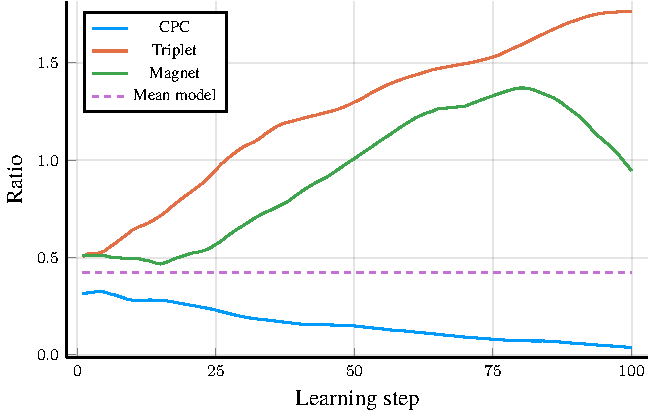
\includegraphics[width=\textwidth]{images/Musk2_ratio/Musk2_ratio.pdf}
    \caption{Musk2, Silhouette coeff.}
  \end{subfigure}
  \begin{subfigure}[t]{0.49\textwidth}
    \centering
    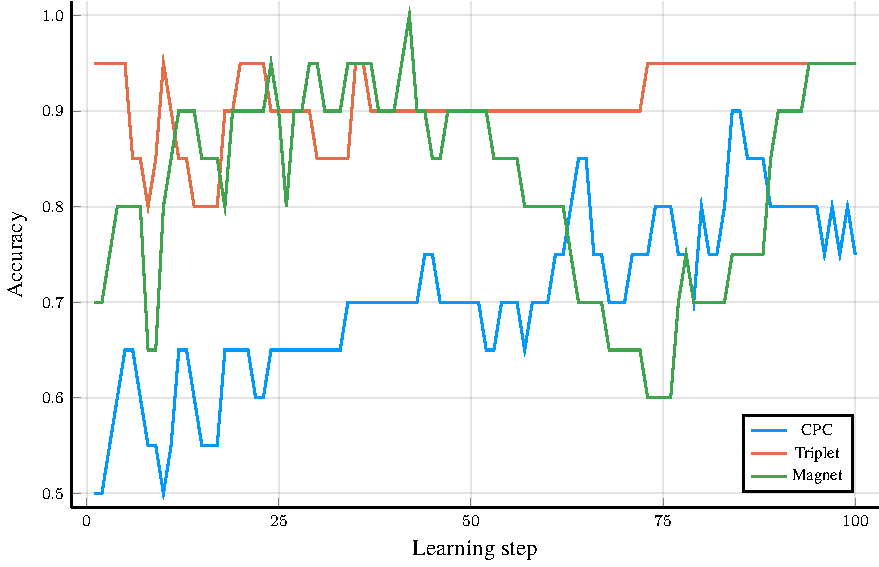
\includegraphics[width=\textwidth]{images/Musk2_accuracy/Musk2_accuracy.pdf}
    \caption{Musk2, accuracy}
  \end{subfigure}
  \begin{subfigure}[t]{0.49\textwidth}
    \centering
    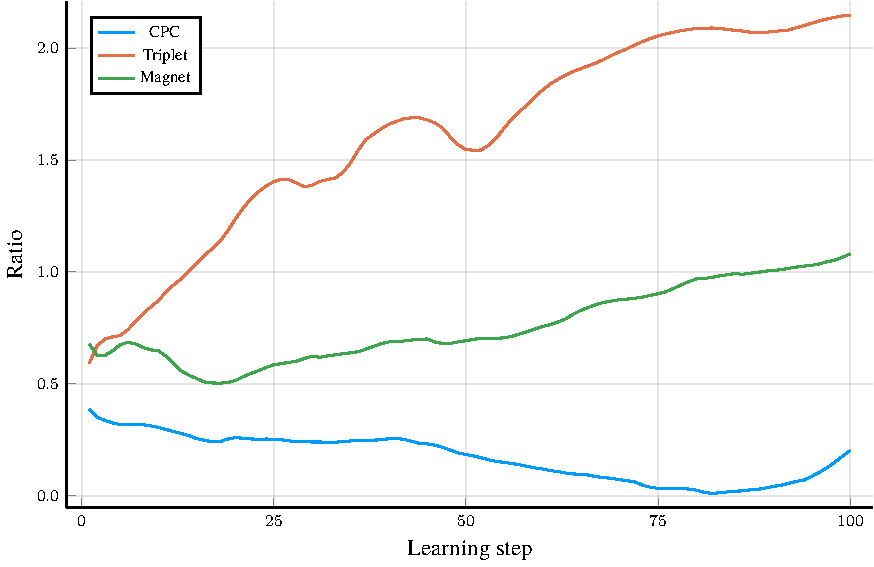
\includegraphics[width=\textwidth]{images/UCSBBreastCancer_ratio/UCSBBreastCancer_ratio.pdf}
    \caption{UCSBBreastCancer, Silhouette coeff.}
  \end{subfigure}
  \begin{subfigure}[t]{0.49\textwidth}
    \centering
    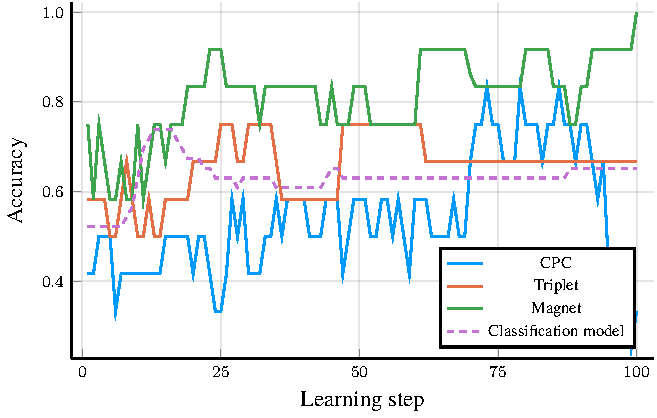
\includegraphics[width=\textwidth]{images/UCSBBreastCancer_accuracy/UCSBBreastCancer_accuracy.pdf}
    \caption{UCSBBreastCancer, accuracy}
  \end{subfigure}
  \begin{subfigure}[t]{0.49\textwidth}
    \centering
    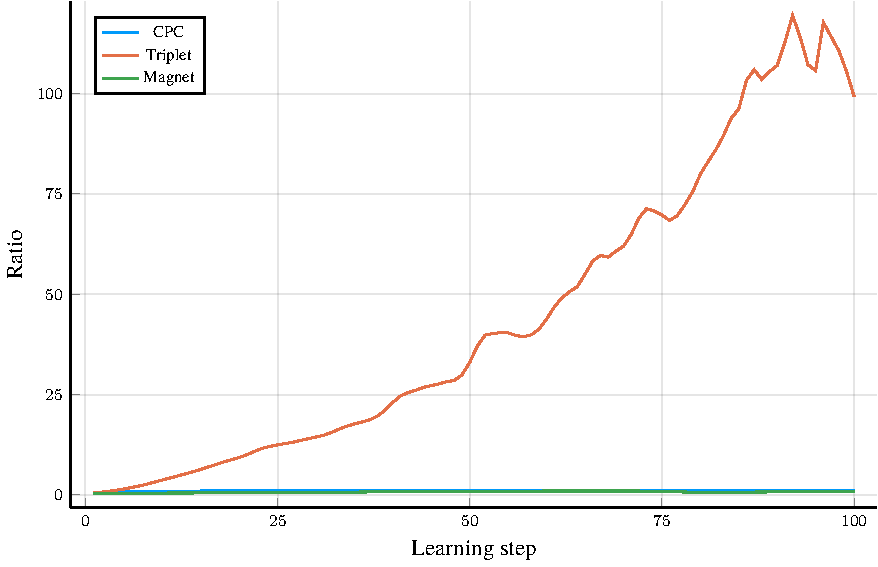
\includegraphics[width=\textwidth]{images/Web3_ratio/Web3_ratio.pdf}
    \caption{Web3, Silhouette coeff.}
  \end{subfigure}
  \begin{subfigure}[t]{0.49\textwidth}
    \centering
    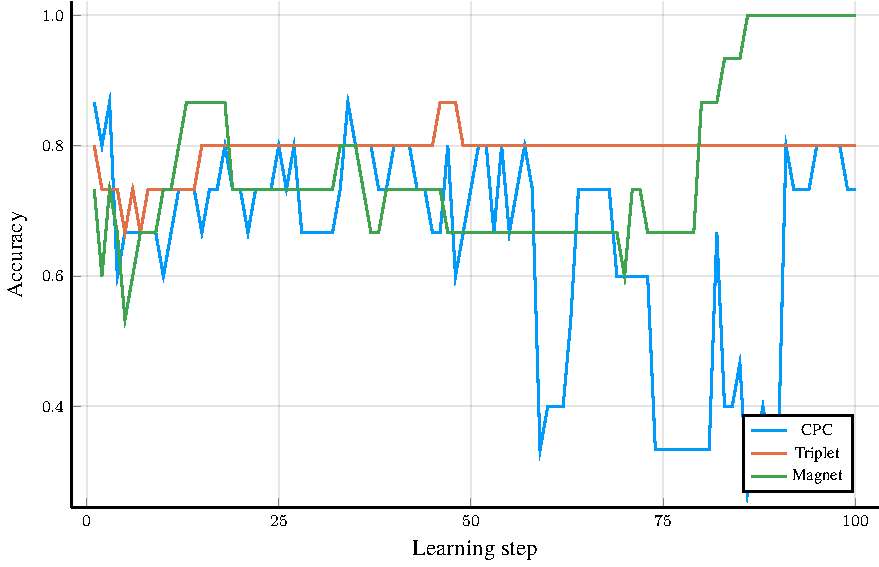
\includegraphics[width=\textwidth]{images/Web3_accuracy/Web3_accuracy.pdf}
    \caption{Web3, accuracy}
  \end{subfigure}
  \caption{Accuracy and the Silhouette coefficient on three selected datasets.}\label{fig:public-comparison}
\end{figure*}

\subsection{Statistical significance of the results}

The null hypothesis that all three methods are the same as measured by the accuracy can be rejected at a 5\% level of significance by the Friedman two-way analysis of variance by ranks \cite{friedman_use_1937}. Triplet and magnet losses are better than CPC at a 5\% level of significance by the post-hoc Nemenyi pairwise test \cite{nemenyi_distribution-free_1963}. However, the null hypothesis that magnet loss and triplet loss are the same cannot be rejected at the 5\% significance level by this test. This further supports the differing results between these two methods as mentioned in the previous subsection.

\subsection{HTTP dataset}

Table~\ref{tab:cisco-accuracy} compares the three methods on the proprietary dataset from Cisco Cognitive Intelligence. Here, magnet loss is the best of the three methods, however, only by a small margin over the other 2 methods. Since the datasets consisted of 90\% of negative samples however, none of the results is particularly remarkable and some further tuning would be needed if any of the methods were to be used in real environment.

\begin{table}
  \centering
  \begin{tabular}{lrrr}
    \toprule
    Variant    & CPC   & Triplet loss & Magnet loss \\
    \midrule
    2 classes  & 0.920 & 0.910        & \textbf{0.930} \\
    20 classes & 0.893 & 0.868        & \textbf{0.904} \\
    \bottomrule
  \end{tabular}
  \caption{The accuracy of the final models for the corporate datasets.}\label{tab:cisco-accuracy}
\end{table}
